%%%%%%%%%%%%%%%%%%%%%%%%%%%%%%%%%%%%%%%%%%%%%%
% curso git y Github para ciencia reproducible
% 1. Introducción
%
% Barcelona, 10-12 Febrero 2025
%
% Urtzi Enriquez-Urzelai 
%%%%%%%%%%%%%%%%%%%%%%%%%%%%%%%%%%%%%%%%%%%%%%


% Inbuilt themes in beamer
\documentclass{beamer}

% additional packages:
\usepackage{minted}
\usepackage[inkscapearea=page]{svg}
\usepackage{caption}
\usepackage{fontawesome}
\usepackage[style=apa]{biblatex}

% Theme choice:
\usetheme{Madrid}
\makeatother
\setbeamertemplate{footline}
{
\leavevmode%
  \hbox{%
  \begin{beamercolorbox}[wd=.2\paperwidth,ht=2.25ex,dp=1.1ex,center]{section in head/foot}%
    \usebeamerfont{section in head/foot}\insertsection
  \end{beamercolorbox}%
  \begin{beamercolorbox}[wd=.8\paperwidth,ht=2.25ex,dp=1.1ex,center]{title in head/foot}%
    \usebeamerfont{title in head/foot}\insertshorttitle\hspace*{24em}
    \insertframenumber{} / \inserttotalframenumber\hspace*{1ex}
  \end{beamercolorbox}}%
}
\makeatletter
\setbeamertemplate{navigation symbols}{}
\setbeamertemplate{caption}[numbered]
\captionsetup[figure]{font=tiny}

% Title page details: 
\section{}
\title{\texttt{git} y \texttt{GitHub} para ciencia reproducible}
\subtitle{1. Introducción}
\author{Urtzi Enriquez-Urzelai\inst{1}}
\institute{ 
    \inst{1} Institute of Vertebrate Biology,
    \newline  
    Czech Academy of Sciences 
    \newline \newline
    \faGithub \hspace*{0.2ex} \href{https://github.com/urtzienriquez}{\color{blue}{GitHub}}
    \hspace*{0.5ex} \faGlobe \hspace*{0.2ex} \href{https://urtzienriquez.github.io/}{\color{blue}{webpage}}
    }
\date{\today}
\logo{
\includegraphics[height=1.0cm,keepaspectratio]{./images/IVB-logo-en-color-big.png}}


\addbibresource{../bib/bib.tex}


\begin{document}

% Title page frame
\begin{frame}
    \titlepage 
\end{frame}

% Remove logo from the rest of frames
\logo{}

% Outline frame
\begin{frame}{Contenido}
    \tableofcontents
\end{frame}


%%% List of frames

% Introducción
\section{Introducción}

\begin{frame}{Ciencia reproducible}
    \begin{figure}
        \centering
        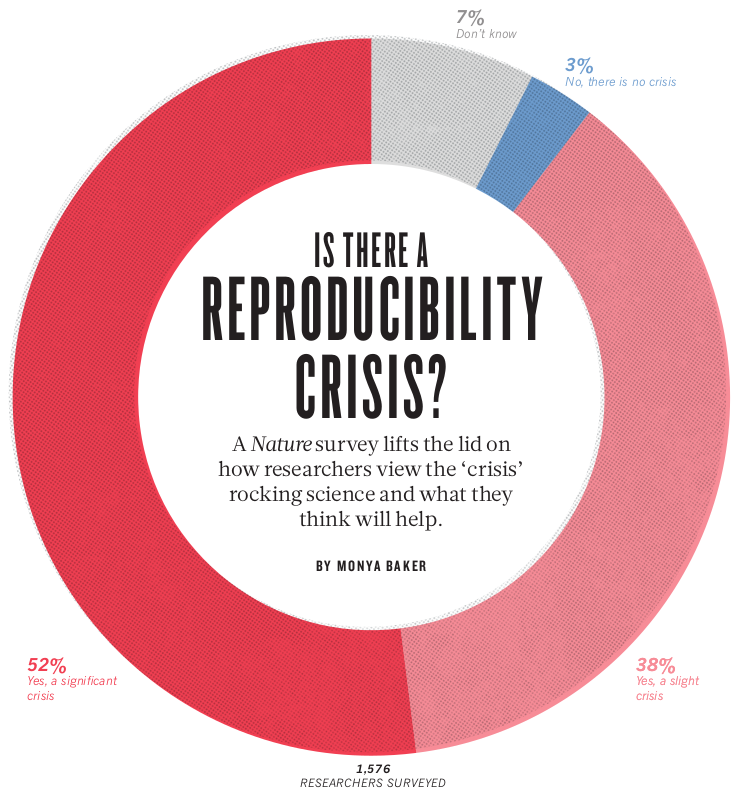
\includegraphics[width=0.55\textwidth]{./images/baker_2016.png}
        \caption{La mayoría de investigadores consideran que hay una 
        crisis de reproducibilidad en ciencia según \textcite{baker2016}.}
    \end{figure}
\end{frame}

\begin{frame}{Ciencia reproducible}
    \begin{columns}
        % Column 1
        \begin{column}{0.5\textwidth}
            \begin{enumerate}
                \item<1-> Información suficiente en 
                \textit{Materiales y Métodos} para poder
                replicar el trabajo.
                \item<2-> Compartir los datos (brutos!)
                \item<3-> Compartir código
            \end{enumerate}
        \end{column}
        % Column 2
        \begin{column}{0.5\textwidth}
            \onslide<4-> 
            \begin{figure}
                \centering
                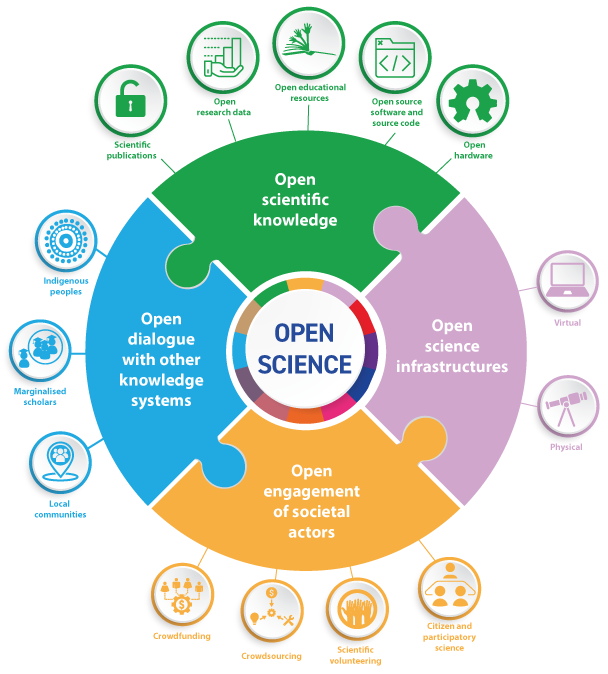
\includegraphics[width=1.0\textwidth]{./images/UNESCO-Open_science-pillars-en.png}
                \caption{Diferentes aspectos para caminar hacia una ciencia abierta
                según la \textcite{unesco2022}.}
            \end{figure}
        \end{column}
    \end{columns}
\end{frame}

\begin{frame}{Ciencia reproducible}
    \begin{figure}
        \centering
        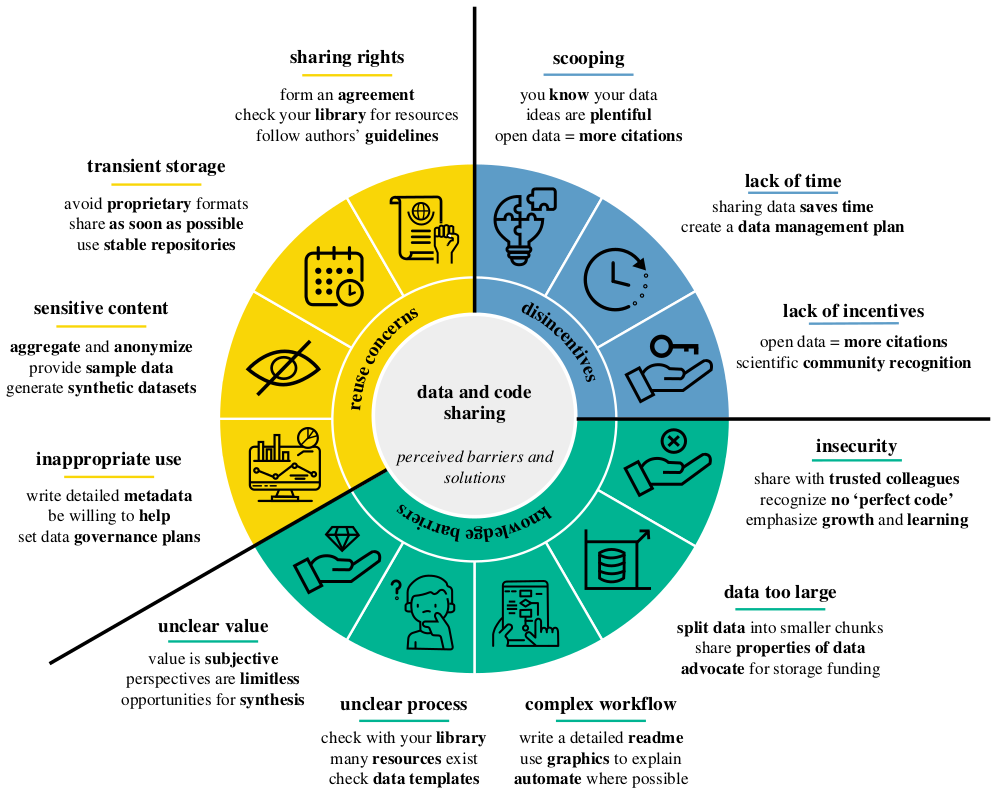
\includegraphics[width=0.73\textwidth]{./images/Gomes_et_al_2022.png}
        \caption{Diferentes impedimentos "aparentes" y los beneficios reales \parencite{gomes2022}.}
    \end{figure}
\end{frame}

\begin{frame}{¿Qué es \texttt{git}?}
    \begin{columns}
        % Column 1
        \begin{column}{0.6\textwidth}
            \texttt{git} es un sistema de control de cambios distribuido, 
            rápido y escalable. \\~\\ \pause
            Registra los cambios hechos sobre archivos
            a lo largo del tiempo. \\~\\ \pause
            \begin{block}{origen}
                \scriptsize
                El creador de \texttt{git} es Linus Torvalds, también conocido 
                por ser el padre de \texttt{Linux}.
            \end{block}
        \end{column}
        % Column 2    
        \begin{column}{0.3\textwidth}
            \begin{figure}
                \centering
                
\includegraphics[width=1.0\textwidth]{./images/git_presentation.png}
                \caption{($arriba$) Linus Torvalds saludando y 
                ($abajo$) el logo de \texttt{git}.}
            \end{figure}
        \end{column}
    \end{columns}
\end{frame}

\begin{frame}{Repositorios}
    \onslide<+-> 
    Cuando trabajamos en \texttt{git}, 
    lo haremos en repositorios.
    \onslide<+-> 
    \begin{columns}
        % Column 1
        \begin{column}{0.6\textwidth}    
            Los repositorios pueden ser:
            \setbeamercovered{transparent}
            \begin{itemize}[<+->]
                \item \textbf{Locales}: almacenados en nuestro ordenador.
                \item \textbf{Remotos}: almacenados en un servidor.
            \end{itemize}
            \setbeamercovered{invisible}
        \end{column} 
        % Column 2    
        \begin{column}{0.3\textwidth}
            \begin{figure}
                    \centering
                    %
\includegraphics[width=0.7\textwidth]{./images/repository-100.png} %no-animation
                    \includegraphics<1-3>[width=0.7\textwidth]{./images/repository-100.png} %animation
                    \includegraphics<4-5>[width=0.7\textwidth]{./images/remote-repository-100.png} %animation                
                    \caption{Representación repositorios.}
            \end{figure}
        \end{column}
    \end{columns}
    \onslide<+-> 
    \begin{block}{ejemplo de servidor}
        \scriptsize
        Hay muchos servidores para almecenar código,
        o cualquier otro tipo de archivos (p.ej. bases
        de datos), pero uno de los servidores más 
        populares para almacenar repositorios es \texttt{GitHub}
    \end{block}
\end{frame}

\begin{frame}{\texttt{Repositorios}}
    \begin{columns}
        % Column 1
        \begin{column}{0.6\textwidth}
            \texttt{GitHub} es el repositorio más conocido para
            almacenar nuestros repositorios. \\~\\ %\pause
            Es propiedad de MicroSoft.
        \end{column} %\pause
        % Column 2    
        \begin{column}{0.3\textwidth}
            \begin{figure}
                \centering
                \includesvg[width=1.0\textwidth]{./images/github-logo.svg}
                \caption{Logo de \texttt{GitHub}.}
            \end{figure}
        \end{column}
    \end{columns}
\end{frame}


% Functionamiento
\section{Funcionamiento}

\begin{frame}{\texttt{Flujo de trabajo}}
    \begin{figure}
        \centering
        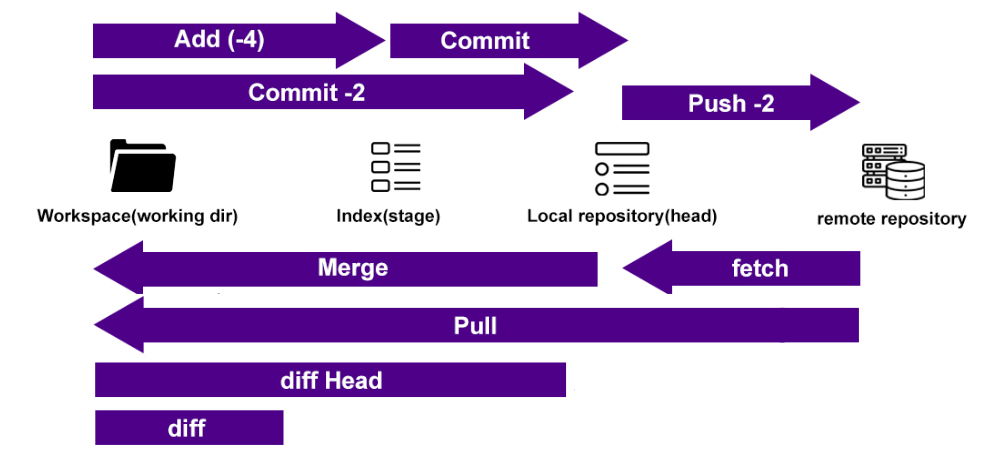
\includegraphics[width=1.0\textwidth]{./images/git-workflow.png}
        \caption{Flujo de trabajo típico de \texttt{git} que muestra 
        las cuatro áreas donde se pueden encontrar nuestros archivos
        y una representación gráfica de los comandos más habituales.
        Imagen obtenida de 
        \href{https://www.geeksforgeeks.org/how-git-version-control-works/}{https://www.geeksforgeeks.org/}}
    \end{figure}
\end{frame}


%% Iniciar un repositorio y commit inicial
\begin{frame}[fragile]{¿Cómo funciona \texttt{git}?}
    \begin{columns}
        % Column 2    
        \begin{column}{0.3\textwidth}
            \begin{figure}
                \centering
                \includesvg[width=1.0\textwidth,keepaspectratio]{./images/func_git_1.svg}
                \caption{\texttt{commit} inicial.}
            \end{figure}
        \end{column}
        % Column 1
        \begin{column}{0.6\textwidth}
            \begin{exampleblock}{código}
                \scriptsize
                \begin{minted}[autogobble]{bash}
                    # Iniciar un repositorio
                    $ git init

                    # Añadir archivos y/o cambios
                    $ git add .

                    # Captura inicial del "estado" de los archivos
                    $ git commit -m "initial commit"

                \end{minted}
            \end{exampleblock}
            \texttt{git init} es la forma de inicializar un repositorio.\newline
            \texttt{git add} indica a \texttt{git} qué archivos o cambios queremos que "traquée".\newline 
            Finalmente, \texttt{git commit} toma una captura (snapshot) de estos cambios 
            en el repositorio local.
        \end{column}
    \end{columns}
\end{frame}

%% Commits
\begin{frame}[fragile]{¿Cómo funciona \texttt{git}?}
    \begin{columns}
        % Column 2    
        \begin{column}{0.3\textwidth}
            \begin{figure}
                \centering
                \includesvg[width=1.0\textwidth,keepaspectratio]{./images/func_git_2.svg}
                \caption{Segundo \texttt{commit}.}
            \end{figure}
        \end{column}
        % Column 1
        \begin{column}{0.6\textwidth}
            \begin{exampleblock}{código}
                \scriptsize
                \begin{minted}[autogobble]{bash}
                    # Capturas secuenciales de los archivos
                    $ git commit -am "fixed some typos"

                    # Incluir los cambios al repositorio remoto
                    $ git push
                \end{minted}
            \end{exampleblock}
            \texttt{git push} sincroniza los cambios realizados localmente con el repositorio remoto. 
        \end{column}
    \end{columns}
\end{frame}

%% Ramas
\begin{frame}[fragile]{¿Cómo funciona \texttt{git}?}
    \begin{columns}
        % Column 2    
        \begin{column}{0.3\textwidth}
            \begin{figure}
                \centering
                \includesvg[width=1.0\textwidth,keepaspectratio]{./images/func_git_3.svg}
                \caption{Nueva rama.}
            \end{figure}
        \end{column}
        % Column 1
        \begin{column}{0.6\textwidth}
            \begin{exampleblock}{código}
                \scriptsize
                \begin{minted}[autogobble]{bash}
                    # consultar qué ramas tenemos
                    $ git branch

                    # crear una nueva rama
                    $ git branch -c new_analysis

                    # movernos a la nueva rama
                    $ git switch new_analysis
                \end{minted}
            \end{exampleblock}
            Las ramas son otro aspecto muy importante de \texttt{git}.\newline
            Trabajar en ramas nos permite modificar código (e.g. desarrollar una
            nueva aplicación o implementar un nuevo análisis) sin interferir con el trabajo
            de otrxs compañerxs.\newline
            Hablaremos más sobre eso mañana. 
        \end{column}
    \end{columns}
\end{frame}

%% Más commits
\begin{frame}[fragile]{¿Cómo funciona \texttt{git}?}
    \begin{columns}
        % Column 2    
        \begin{column}{0.3\textwidth}
            \begin{figure}
                \centering
                \includesvg[width=1.0\textwidth,keepaspectratio]{./images/func_git_4.svg}
                \caption{Más \texttt{commit}s.}
            \end{figure}
        \end{column}
        % Column 1
        \begin{column}{0.6\textwidth}
            Continuaremos trabajando tanto en la rama principal, como en otras ramas y
            haremos capturas (i.e. \texttt{git commit}) en puntos estratégicos.
        \end{column}
    \end{columns}
\end{frame}

%% Merge
\begin{frame}[fragile]{¿Cómo funciona \texttt{git}?}
    \begin{columns}
        % Column 2    
        \begin{column}{0.3\textwidth}
            \begin{figure}
                \centering
                \includesvg[width=1.0\textwidth,keepaspectratio]{./images/func_git_5.svg}
                \caption{Fusionar ramas.}
            \end{figure}
        \end{column}
        % Column 1
        \begin{column}{0.6\textwidth}
            \begin{exampleblock}{código}
                \scriptsize
                \begin{minted}[autogobble]{bash}
                    # movernos a la rama principal
                    $ git switch main

                    # fusionar las ramas
                    $ git merge new_analysis
                \end{minted}
            \end{exampleblock}
            En algún punto, el trabajo realizado en una rama podrá ser fusionado con 
            la rama principal \textemdash o con cualquier otra rama\textemdash, p. ej.
            cuando el nuevo análisis esté ya preparado y funcionando.  
        \end{column}
    \end{columns}
\end{frame}


% Aplicaciones
\section{Aplicaciones}

\begin{frame}<1>[label=frame_ref]{Aplicaciones de \texttt{GitHub}}
    \setbeamercovered{transparent}
    \textbf{Almacenar} remotamente y registrar los cambios de:
    \begin{enumerate}
        \item<1-> Bases de datos
        \item<2-> Código fuente de programas
        \item<3-> \textit{Scripts} de análisis
        \item<4-> Código completo para reproducir artículos científicos
    \setbeamercovered{invisible}
    \end{enumerate}
\end{frame}

% ejemplo: bases de datos
\frame[noframenumbering]{
    \frametitle{Aplicaciones de \texttt{GitHub}}
    \href{https://github.com/jslucassf/geoinfo-spatial-relations/}{\color{blue}{https://github.com/jslucassf/geoinfo-spatial-relations/}}
    \begin{figure}
        \centering
        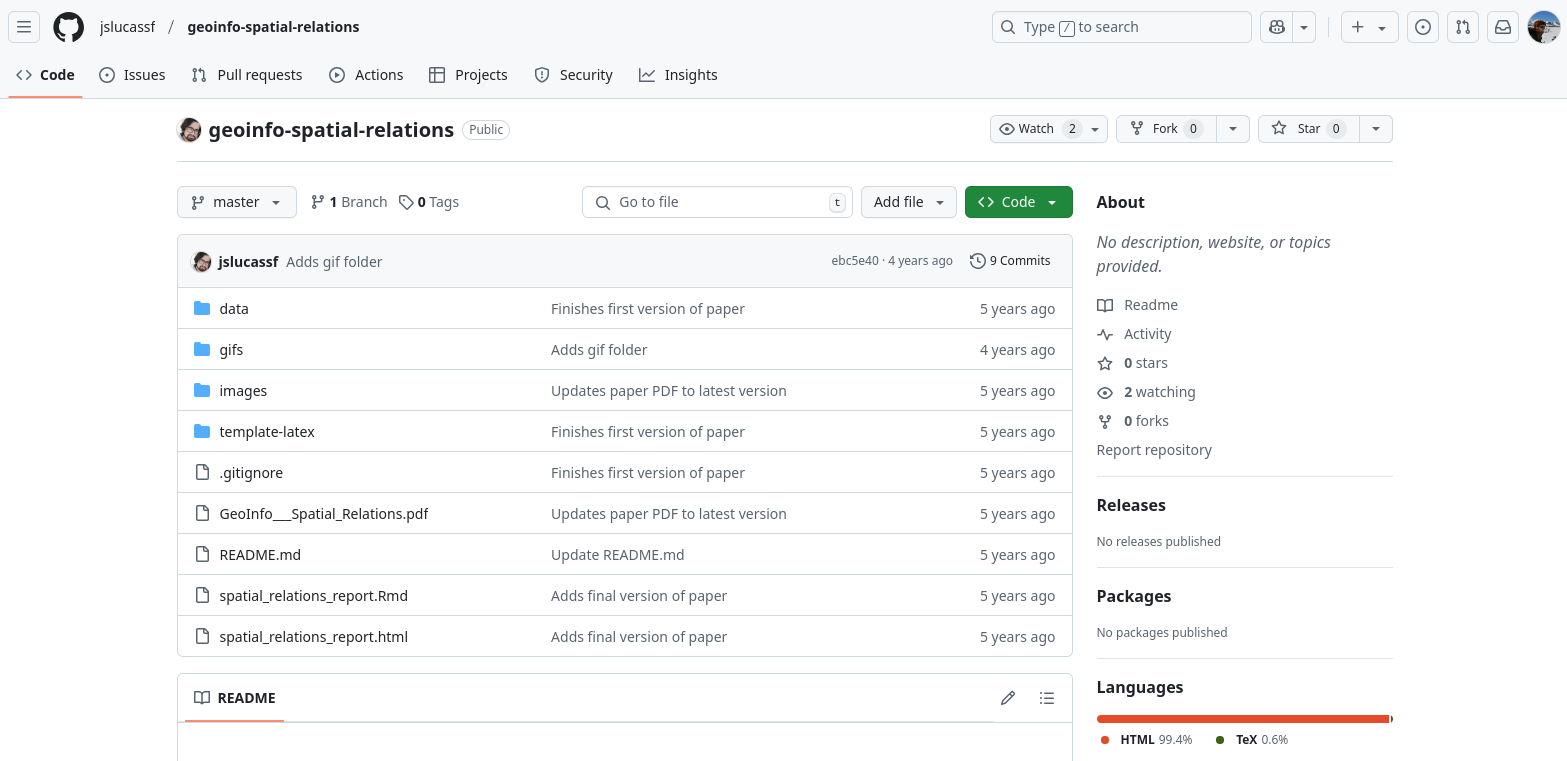
\includegraphics[width=1.0\textwidth,keepaspectratio]{./images/ex_repo1.png}
    \end{figure}
}
\addtocounter{framenumber}{-1}
\againframe<2>{frame_ref}

% ejemplo: Código fuente de programas
\frame[noframenumbering]{
    \frametitle{Aplicaciones de \texttt{GitHub}}
    \href{https://github.com/mrke/NicheMapR}{\color{blue}{https://github.com/mrke/NicheMapR}}
    \begin{figure}
        \centering
        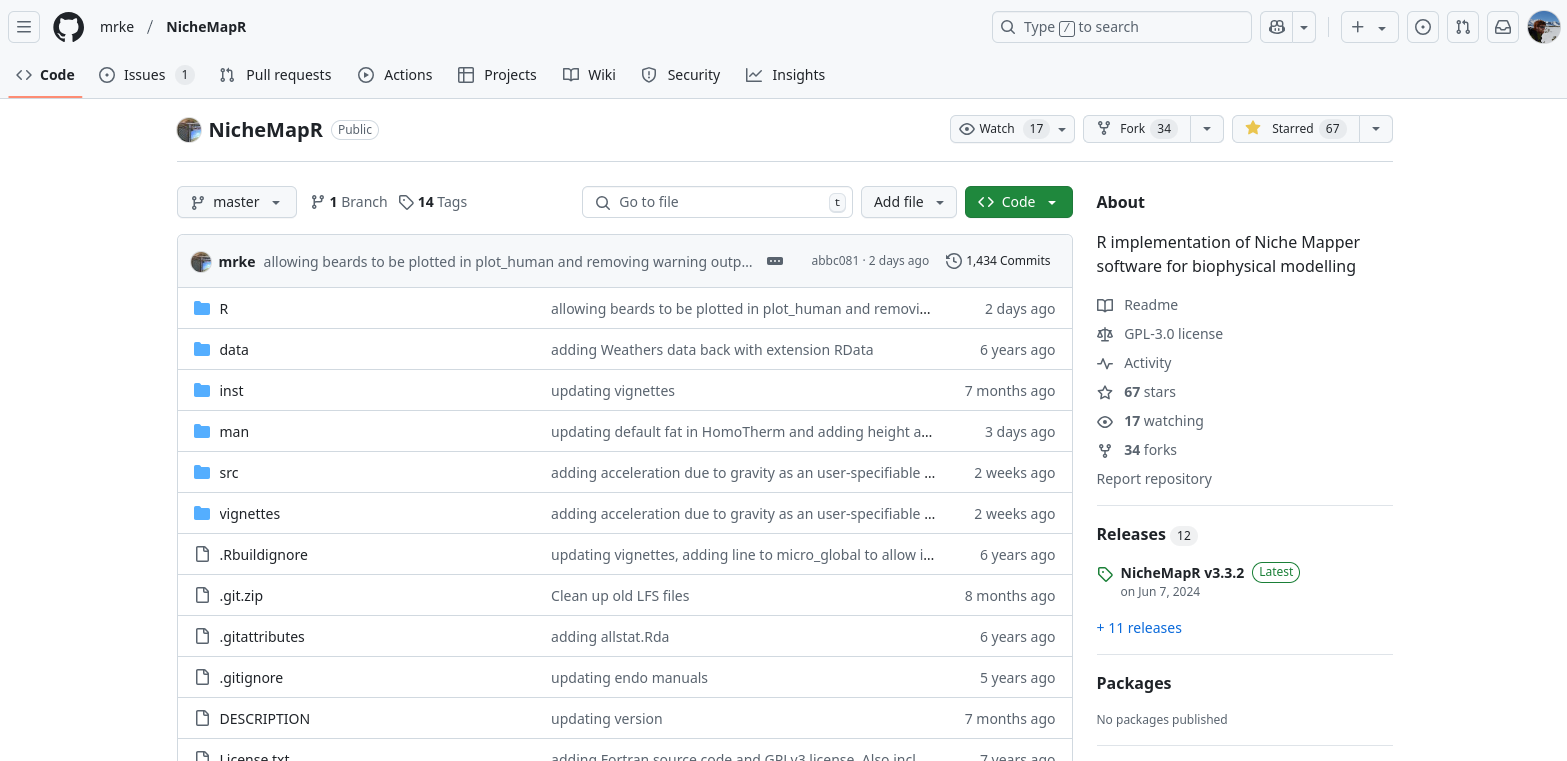
\includegraphics[width=1.0\textwidth,keepaspectratio]{./images/ex_repo2.png}
    \end{figure}
}
\addtocounter{framenumber}{-1}
\againframe<3>{frame_ref}

% ejemplo: Scripts de análisis
\frame[noframenumbering]{
    \frametitle{Aplicaciones de \texttt{GitHub}}
    \href{https://github.com/helenamartg/Rana}{\color{blue}{https://github.com/helenamartg/Rana}}
    \begin{figure}
        \centering
        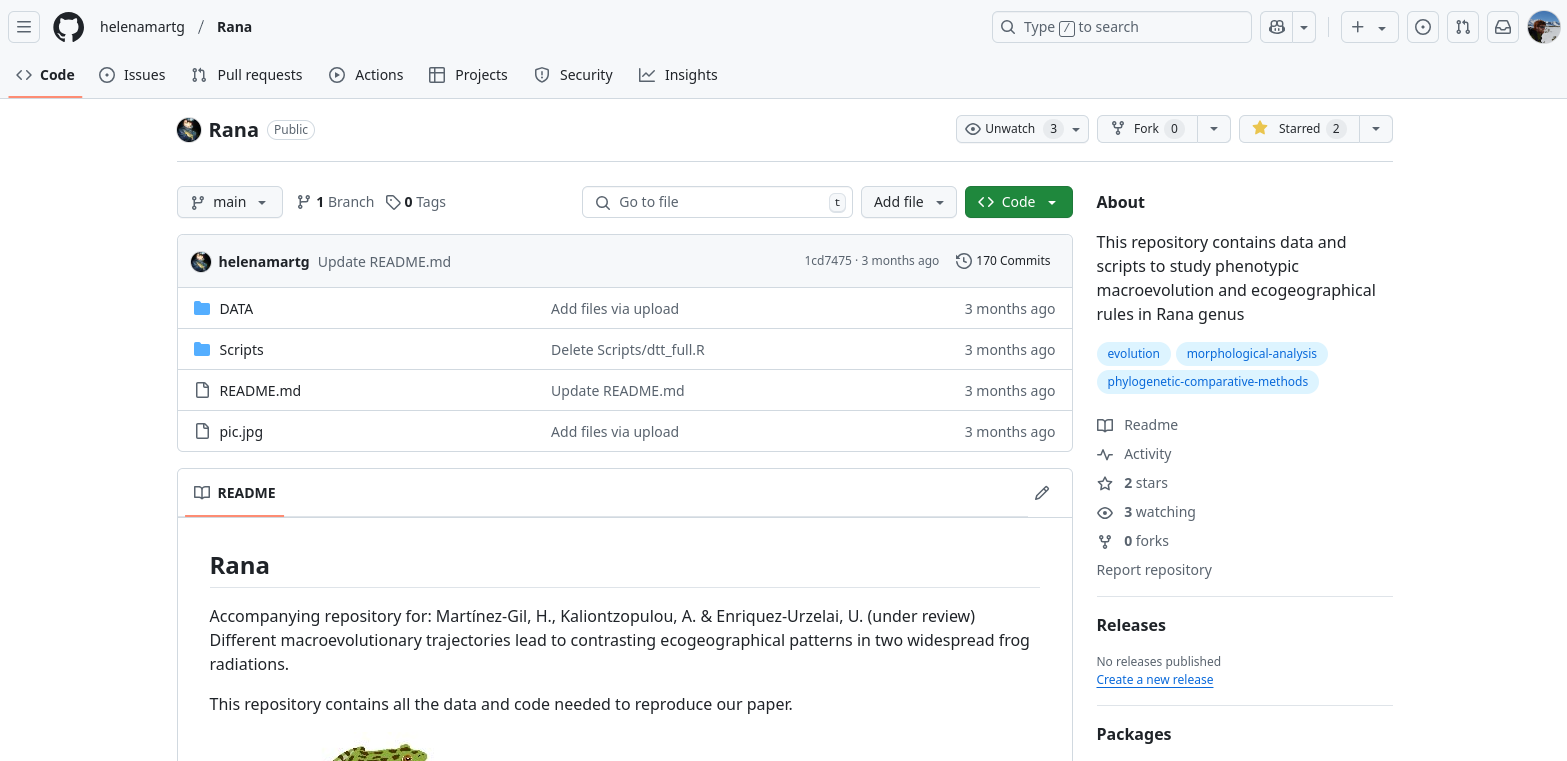
\includegraphics[width=1.0\textwidth,keepaspectratio]{./images/ex_repo3.png}
    \end{figure}
}
\addtocounter{framenumber}{-1}
\againframe<4>{frame_ref}

% ejemplo: Código completo para reproducir artículos científicos
\frame[noframenumbering]{
    \frametitle{Aplicaciones de \texttt{GitHub}}
    \href{https://github.com/urtzienriquez/ThermHydroBehav/}{\color{blue}{https://github.com/urtzienriquez/ThermHydroBehav/}}
    \begin{figure}
        \centering
        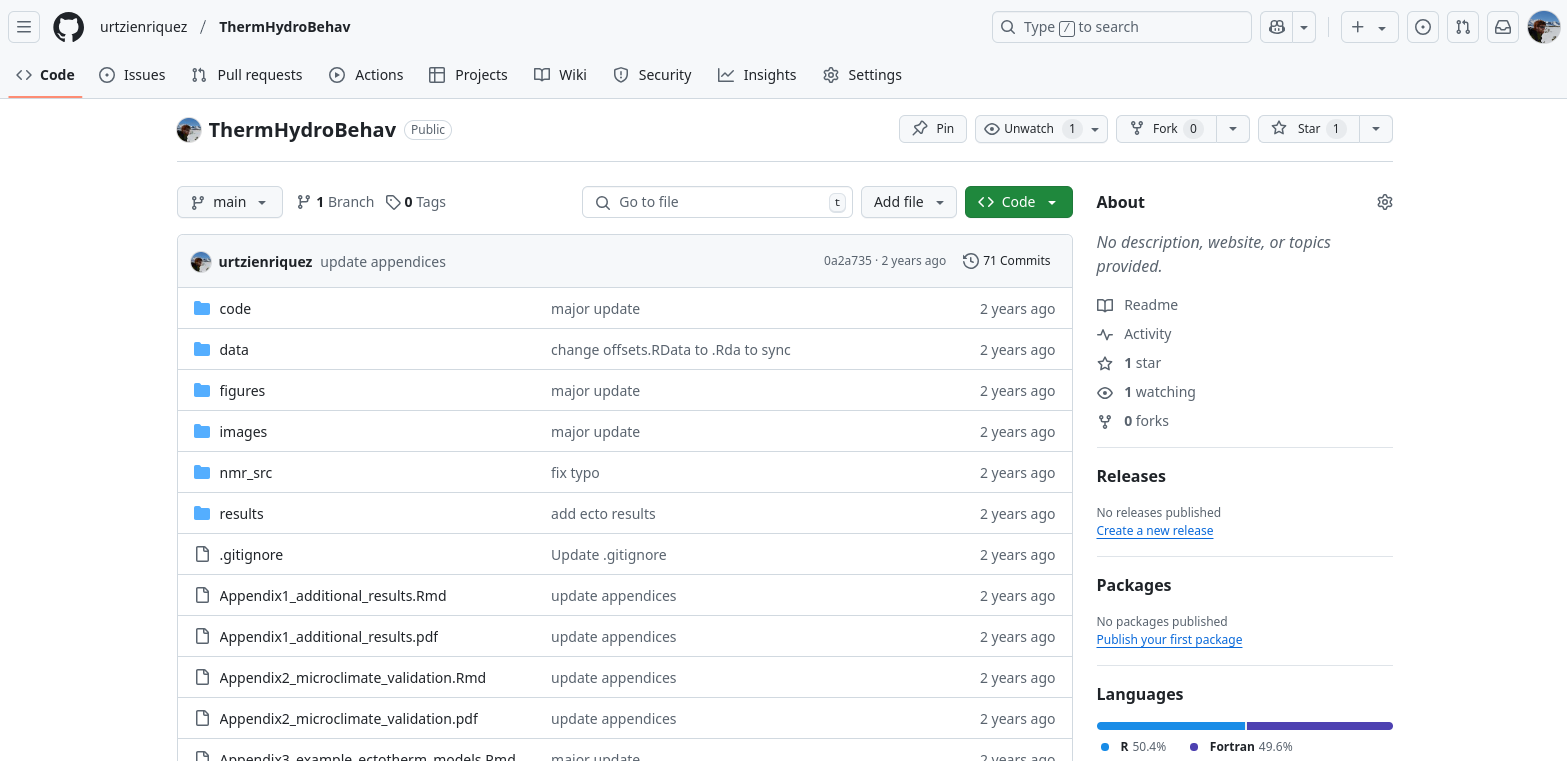
\includegraphics[width=1.0\textwidth,keepaspectratio]{./images/ex_repo4.png}
    \end{figure}
}


% Referencias
\section{Referencias}

\begin{frame}{Referencias}
    \printbibliography
\end{frame}


% Puesta a punto; instalación 
\section{Puesta a punto}

\begin{frame}{Puesta a punto}
    Vamos a necesitar: 
    \begin{enumerate}
        \item Instalar git (\href{https://git-scm.com/downloads}{\color{blue}{https://git-scm.com/downloads}})
        \item Crear una cuenta en GitHub (\href{https://github.com/}{\color{blue}{https://github.com/}})
        \item Instalar GitHub Desktop (\href{https://desktop.github.com/download/}{\color{blue}{https://desktop.github.com/download/}})
        \item Editor de texto (e.g. notepad, RStudio o VSCode) \\~\\
    \end{enumerate}
    Opcional para el artículo reproducible: 
    \begin{enumerate}
        \item R (\href{https://cran.r-project.org/}{\color{blue}{https://cran.r-project.org/}})
        \item y los paquetes de R:
        \begin{enumerate}
            \item rmarkdown 
            \item knitr
        \end{enumerate} 
        \item pandoc
        \item \LaTeX
    \end{enumerate}
\end{frame}


\end{document}